\chapter{Détection de rupture}

\section{Introduction}

Cette partie présentera les deux méthodes de détection de rupture implémentées : une méthode par dérivée filtrée utilisant la $p$-valeur décrite par \cite{Bertrand11} et \cite{Herault14}, et une méthode de détection de changement de noyau décrite par \cite{Desobry05}.

Cette détection de rupture sera appliquée sur une matrice de signal $X$ contenant $n$ lignes d'« observations », une par image de la vidéo, et $p$ colonnes de caractéristiques, 1 pour chaque caractéristique extraite de la vidéo.

\demoinfo{Ce chapitre est accompagné de démonstrations, qui prennent la forme de blocs de code Matlab dans le fichier \emph{Projet.m}. Des paragraphes identiques à celui-ci indiqueront quels blocs de code correspondent aux sections du rapport.}

\section{Prétraitement des caractéristiques}

Avant de se lancer dans la détection, il peut être intéressant de regarder ce que contient la matrice de caractéristiques $X$. On se propose de la visualiser sous la forme d'une image représenté par la figure \ref{Xorigin}.

Notons que cette première matrice contient des blocs de caractéristiques superposés verticalement (RGB puis YCbCr puis coocurence, etc.), et que chacun de ces blocs a été normalisé entre 0 et 1 afin que les caractéristiques soient comparables entre elles.

On peut voir sur la figure qu'à première vue, la matrice à l'air quasiment creuse, comme si tout valait $0$. En réalité, cette perception est due au fait que quelques composantes de chacune des caractéristiques prend des très grandes valeurs. Par exemple sur une image noire, certaines caractéristiques prennent des très grandes valeurs comparativement aux autres.

On se propose donc de prétraiter cette matrice $X$ par une fonction de normalisation appliquée à chaque valeur de la matrice. 

\demoinfo{Les blocs 1 \& 2 de la démonstration permettent de tester diverses fonctions de normalisation dans une figure interractive.}

Finalement, on retiendra la fonction de normalisation $\log (10^9 X + 1)$ donnant le résultat visible en figure \ref{Xpreprocessed}, sur laquelle les valeurs des caractéristiques apparaissent bien plus clairement.

\begin{figure} [h]
\centering
	\begin{subfigure}[b]{0.6\textwidth}
		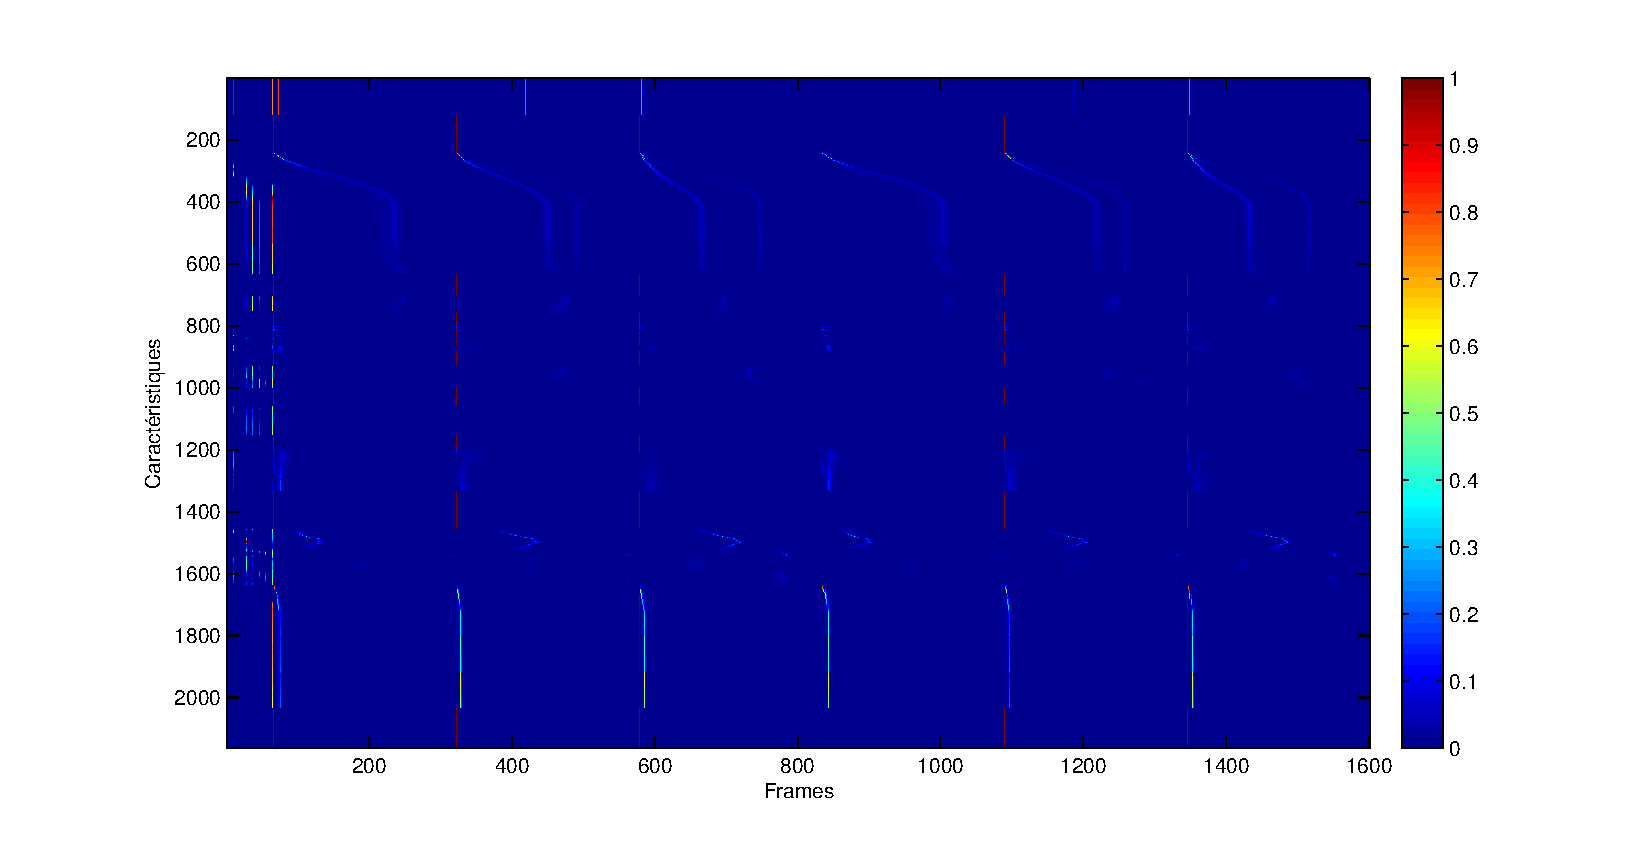
\includegraphics[width=\textwidth]{images/signal}
		\caption{Matrice $X$ originale}
		\label{Xorigin}
    \end{subfigure} \\
	\begin{subfigure}[b]{0.6\textwidth}
		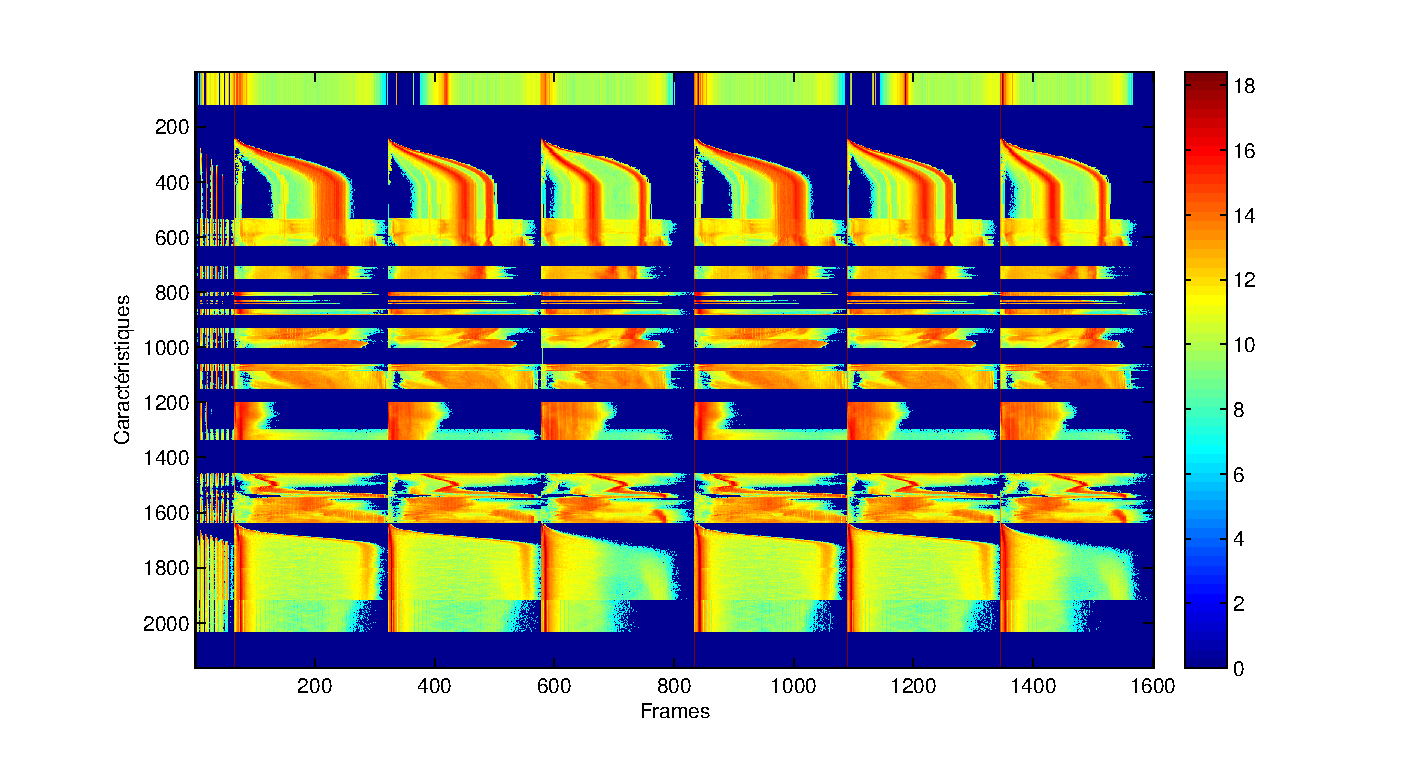
\includegraphics[width=\textwidth]{images/signalPreprocessed}
		\caption{Matrice $X$ prétraitée}
		\label{Xpreprocessed}
    \end{subfigure}
    \caption{Matrices $X$ avant et après prétraitement}
\end{figure}

\section{Principe de la dérivée filtrée}

\subsection{Méthode de la dérivée filtrée}

Le principe de la méthode utilisée est de parcourir le signal temporel $X$ avec deux fenêtres de taille $A_1$ et $A_2$ respectivement avant et après une position $k$ (de $k - A_1$ à $k-1$ et de $k$ à $k+A_2-1$).

On calcule ensuite, pour chaque position $k$, une valeur de distance $D(k)$ entre des indicateurs $\hat{\theta}$ calculés sur chaque fenêtre.

On détermine ensuite les zones de rupture comme étant les zones telles que $|D(k)| > C$, avec $C$ un seuil fixé, puis on détermine pour chaque zone de rupture $\mathcal{K}_i$ la position $k_{r_i}$ exacte de la rupture comme étant $k_{r_i} = \displaystyle \argmax_{k \in \mathcal{K}_i} |D(k)|$.

\subsection{Calcul de $C$ de façon probabiliste}

Afin de déterminer le seuil $C$, il est possible d'utiliser une méthode probabiliste utilisant la $p$-valeur. En posant $M = \displaystyle \max_{k} |D(k)|$, et l'hypothèse $\mathcal{H}_0$ où il n'y a pas de rupture, on veut $C$ tel que $\mathbb{P}(M>C\mid	\mathcal{H}_0) < p$ avec $p$ fixé.

Pour estimer $C$, on calcule des estimations de réalisation de $M$ sous l'hypothèse $\mathcal{H}_0$ en permutant le signal temporel $X$ (cela force en quelque sorte $\mathcal{H}_0$) et en calculant $\hat{M}$ sur ce nouveau signal. Ces réalisations $\hat{M}$ permettent d'estimer la distribution de $M$. En supposant qu'il s'agisse d'une loi normale, on peut estimer ses paramètres $\hat{\mu}$ et $\hat{\sigma}$, et on peut ainsi estimer le seuil $C$ en fonction d'une valeur fixée de $p$.

\section{Changement de noyau}

La méthode de détection de changement de noyau est un cas particulier de la méthode de la dérivée filtrée où la distance $D(k)$ est calculée comme étant une distance entre les paramètres $\rho_i$ et $\alpha_i$ de deux \textit{one-class SVM} calculés respectivement sur chaque fenêtre (les $\hat{\theta}$ estimés sur chaque fenêtre).

Dans ce cas, pour chaque valeur de $k$, la distance est la suivante :

\begin{align}
  D &= \frac{\overset{\frown}{c_1 c_2}}{\overset{\frown}{c_1 p_1} + \overset{\frown}{c_2 p_2}} \notag \\
  \overset{\frown}{c_1 c_2} &= \arccos\left(\frac{
  	\alpha_1^\top K_{12} \alpha_2
  	}{
  	\sqrt{\alpha_1^\top K_{11} \alpha_1} \sqrt{\alpha_2^\top K_{22} \alpha_2}
  	} \right) \notag \\
  \overset{\frown}{c_i p_i} &= \arccos\left( \frac{\rho_i}{\sqrt{\alpha_i^\top K_{ii} \alpha_i}}  \right) \notag
\end{align}

avec $i$ et $j$ le numéro du \textit{one-class SVM}, $\alpha_i$ les variables duales, $\rho_i$ le biais et $K_{ij}$ la matrice de Gram avec les données $i$ et $j$.

\section{Implémentation}

Ces méthodes de détection de rupture ont été appliquées à la première bande-annonce du film \textit{Star Wars 7}. Cette section présentera les résultats de détection de rupture obtenus sur la matrice de caractéristiques prétraitée de cette vidéo, visible en figure \ref{Xpreprocessed}.

\subsection{Distances}

La méthode de la dérivée filtrée a donc été essayée avec deux distances et estimateurs différents :

\begin{enumerate}
\item Somme des différences absolues entre moyennes ($\hat{\theta}_i = \bar{X}_{k,A_i}$, $D(k) = \sum |\hat{\theta}_1 - \hat{\theta}_2|$)
\item Différence de noyaux
\end{enumerate}

Ces distances seront nommées \textit{distance moyenne} et \textit{distance SVM} par la suite.

\subsection{Choix des fenêtres $A_i$}

Les premiers paramètres à fixer sont des tailles des fenêtres avec lesquelles on parcourt le signal.

Pour cela, nous avons choisi de réaliser une figure interactive permettant de visualiser la distance obtenue avec la \textit{distance moyenne}, en fonction des fenêtres. Ce résultat est affiché sur un graphique indiquant les vraies ruptures dans la vidéo (étiquetées manuellement) afin de pouvoir comparer la distance aux ruptures.

Les fenêtres ont donc été choisies manuellement en deux passes. Tout d'abord on fait varier $A_1$ et on impose $A_2 = A_1$. Puis on fixe $A_1$ avec la valeur choisie précédemment (dans notre cas $A_1=20$) et on fait varier $A_2$ afin de choisir la meilleure valeur (dans notre cas $A_2=28$).

\demoinfo{Le code permettant de choisir $A_1$ correspond au bloc 3 de la démonstration, et celui de $A_2$ au bloc 4.}

\subsection{Choix de $C$}

Normalement, il est possible de choisir la valeur $C$ par la méthode présentée précédemment. Cependant, dans notre cas, compte tenu du nombre de caractéristiques et d'images dans la vidéo, la permutation aléatoire des images de la vidéo demande beaucoup de ressources (5 minutes environ pour 200 permutations).

Or, cette méthode nécessite énormément de permutations pour être efficace. En effet, avec les 200 permutations effectuées, la méthode nous donne pour $p=0$ (valeur extrême qui ne devrait engendrer aucun faux-positif) un $C=0,46$ avec la \textit{distance moyenne}, alors même que ce seuil entraîne beaucoup de faux positifs et que le seuil idéal se situe plutôt autour de $C=0,6$ d'après les graphiques de distance vus durant le choix des $A_i$.

On choisira donc $C$ manuellement, avec $C=0,6$ pour la \textit{distance moyenne} et $C=0,8$ pour la \textit{distance SVM}.

\demoinfo{Le bloc 5 de la démonstration montre l'évolution de $C$ en fonction de $p$, permettant de voir que les valeurs de $C$ ne « montent » pas suffisamment haut.}

\subsection{Résultats}

On obtient finalement les résultats de détection représentés en figure \ref{resMoy} pour la \textit{distance moyenne} et la figure \ref{resSVM} pour la \textit{distance SVM}. On observe quelques erreurs mais le résultat est globalement satisfaisant.

\demoinfo{Ces résultats peuvent être observés dans des figures interractives permettant de visualiser la vidéo autour de chaque rupture. Ce code correspond aux blocs 6 et 7.}

\begin{figure}
\centering
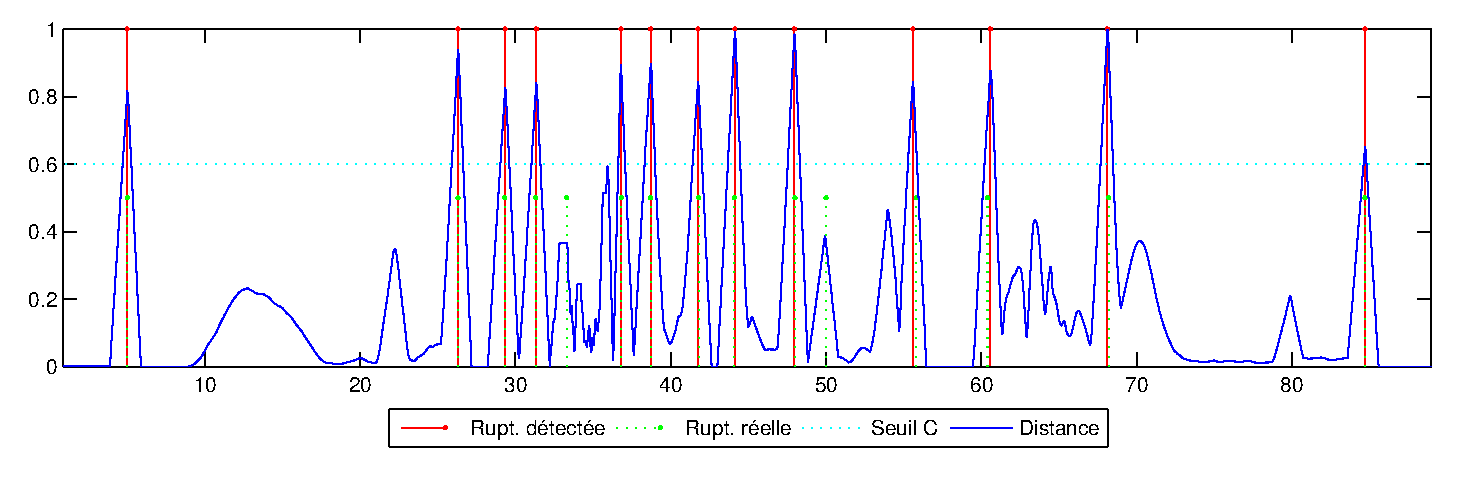
\includegraphics[width=\textwidth]{images/resultatMoy}
\caption{Résultat avec la \textit{distance moyenne}}
\label{resMoy}
\end{figure}


\begin{figure}
\centering
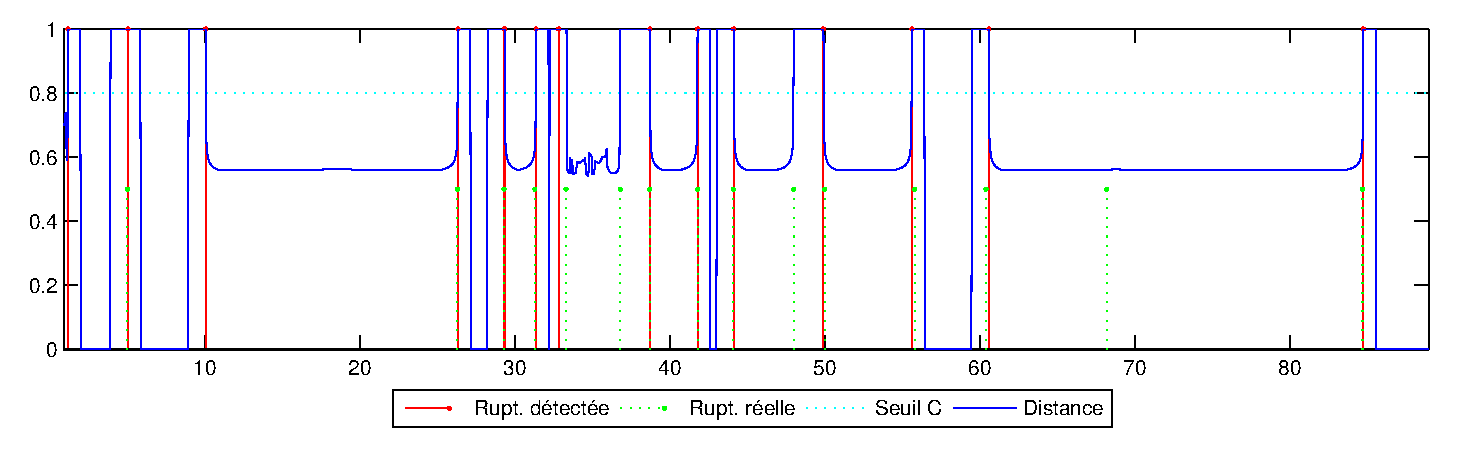
\includegraphics[width=\textwidth]{images/resultatSVM}
\caption{Résultats avec la \textit{distance SVM}}
\label{resSVM}
\end{figure}

\nocite{Loosli05}
